\documentclass[tikz, border=2pt]{standalone}
\usepackage{tikz}
\begin{document}
    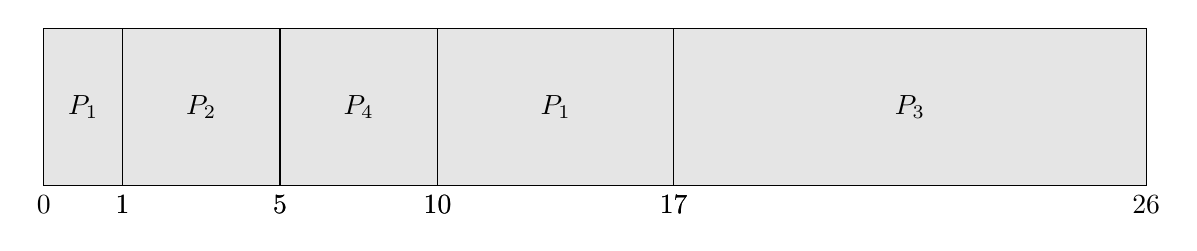
\begin{tikzpicture}
        \draw [fill=gray!20] (0,0) rectangle (1,2)
            node [midway] {$P_1$}
            node [pos=0, below] {0}
            node at (1,0) [below] {1};
        \draw [fill=gray!20] (1,0) rectangle (3,2)
            node [midway] {$P_2$}
            node [pos=0, below] {1}
            node at (3,0) [below] {5};
        \draw [fill=gray!20] (3,0) rectangle (5,2)
            node [midway] {$P_4$}
            node [pos=0, below] {5}
            node at (5,0) [below] {10};
        \draw [fill=gray!20] (5,0) rectangle (8,2)
            node [midway] {$P_1$}
            node [pos=0, below] {10}
            node at (8,0) [below] {17};
        \draw [fill=gray!20] (8,0) rectangle (14,2)
            node [midway] {$P_3$}
            node [pos=0, below] {17}
            node at (14,0) [below] {26};
    \end{tikzpicture}
\end{document}